%%
%% This is file `acmtog.tex',
%% generated with the docstrip utility.
%%
%% The original source files were:
%%
%% samples.dtx  (with options: `all,acmtog')
%% 
%% IMPORTANT NOTICE:
%% 
%% For the copyright see the source file.
%% 
%% Any modified versions of this file must be renamed
%% with new filenames distinct from acmtog.tex.
%% 
%% For distribution of the original source see the terms
%% for copying and modification in the file samples.dtx.
%% 
%% This generated file may be distributed as long as the
%% original source files, as listed above, are part of the
%% same distribution. (The sources need not necessarily be
%% in the same archive or directory.)
%%
%%
%% Commands for TeXCount
%TC:macro \cite [option:text,text]
%TC:macro \citep [option:text,text]
%TC:macro \citet [option:text,text]
%TC:envir table 0 1
%TC:envir table* 0 1
%TC:envir tabular [ignore] word
%TC:envir displaymath 0 word
%TC:envir math 0 word
%TC:envir comment 0 0
%%
%% The first command in your LaTeX source must be the \documentclass
%% command.
%%
%% For submission and review of your manuscript please change the
%% command to \documentclass[manuscript, screen, review]{acmart}.
%%
%% When submitting camera ready or to TAPS, please change the command
%% to \documentclass[sigconf]{acmart} or whichever template is required
%% for your publication.
%%
%%
\documentclass[acmtog,nonacm]{acmart}
%%
\usepackage{acro}
\usepackage{tabularx}
\DeclareAcronym{AAC}{
  short = AAC,
  long  = Architecture-as-Code
}

\DeclareAcronym{AD}{
  short = AD,
  long  = Architecture Description
}

\DeclareAcronym{ADL}{
  short = ADL,
  long  = Architecture Description Language
}

\DeclareAcronym{AI}{
  short = AI,
  long  = Artificial Intelligence
}

\DeclareAcronym{AKS}{
  short = AKS,
  long  = Azure Kubernetes Service
}

\DeclareAcronym{CSA}{
  short = CSA,
  long  = European Union Cybersecurity Act
}

\DeclareAcronym{CSIRT}{
  short = CSIRT,
  long  = Computer Security Incident Response Team
}

\DeclareAcronym{DORA}{
  short = DORA,
  long  = Digital Operational Resilience Act
}

\DeclareAcronym{DSL}{
  short = DSL,
  long  = Domain Specific Language
}

\DeclareAcronym{DSRM}{
  short = DSRM,
  long  = Design Science Research Methodology
}

\DeclareAcronym{EA}{
  short = EA,
  long  = Enterprise Architecture
}

\DeclareAcronym{eIDAS2}{
  short = eIDAS2,
  long  = {Electronic Identification, Authentication and Trust Services}
}

\DeclareAcronym{ENISA}{
  short = ENISA,
  long  = European Union Agency for Cybersecurity
}

\DeclareAcronym{EoI}{
  short = EoI,
  long  = Entity of Interest
}

\DeclareAcronym{EU}{
  short = EU,
  long  = European Union
}

\DeclareAcronym{GenAI}{
  short = GenAI,
  long  = Generative Artificial Intelligence
}

\DeclareAcronym{HTML}{
  short = HTML,
  long  = HyperText Markup Language
}

\DeclareAcronym{ICT}{
  short = ICT,
  long  = Information and Communication Technology
}

\DeclareAcronym{ID}{
  short = ID,
  long  = Identifier
}

\DeclareAcronym{ITS}{
  short = ITS,
  long  = Implementing Technical Standards
}

\DeclareAcronym{LLM}{
  short = LLM,
  long  = Large Language Model
}

\DeclareAcronym{MAD}{
  short = MAD,
  long  = Multi-agent debate
}

\DeclareAcronym{MURCIA}{
  short = MURCIA,
  long  = MUlti-layered Regulatory Change Identification and Analysis
}

\DeclareAcronym{NIS2}{
  short = NIS2,
  long  = Network and Information Systems
}

\DeclareAcronym{NIST}{
  short = NIST,
  long  = National Institute of Standards and Technology
}

\DeclareAcronym{NLP}{
  short = NLP,
  long  = Natural Language Processing
}

\DeclareAcronym{RAG}{
  short = RAG,
  long  = Retrieval-Augmented Generation
}

\DeclareAcronym{RE}{
  short = RE,
  long  = Requirements Engineering
}

\DeclareAcronym{RTS}{
  short = RTS,
  long  = Regulatory Technical Standards
}

\DeclareAcronym{TFEU}{
  short = TFEU,
  long  = Treaty on the Functioning of the European Union
}

\DeclareAcronym{TLPT}{
  short = TLPT,
  long  = Threat-Led Penetration Tests
}

\DeclareAcronym{TOGAF}{
  short = TOGAF,
  long  = The Open Group Architecture Framework
}

\DeclareAcronym{UML}{
  short = UML,
  long  = Unified Modelling Language
}

\DeclareAcronym{XML}{
  short = XML,
  long  = Extensible Markup Language
}



\DeclareAcronym{IT}{
  short = IT,
  long  = Information Technologies
}

%% \BibTeX command to typeset BibTeX logo in the docs
\AtBeginDocument{%
  \providecommand\BibTeX{{%
    Bib\TeX}}}

%% Rights management information.  This information is sent to you
%% when you complete the rights form.  These commands have SAMPLE
%% values in them; it is your responsibility as an author to replace
%% the commands and values with those provided to you when you
%% complete the rights form.
%\setcopyright{acmlicensed}
%\copyrightyear{2018}
%\acmYear{2018}
%\acmDOI{XXXXXXX.XXXXXXX}

%% These commands are for a JOURNAL article.
%\acmJournal{TOG}
%\acmVolume{37}
%\acmNumber{4}
%\acmArticle{111}
%\acmMonth{8}

%%
%% Submission ID.
%% Use this when submitting an article to a sponsored event. You'll
%% receive a unique submission ID from the organizers
%% of the event, and this ID should be used as the parameter to this command.
%%\acmSubmissionID{123-A56-BU3}

%%
%% For managing citations, it is recommended to use bibliography
%% files in BibTeX format.
%%
%% You can then either use BibTeX with the ACM-Reference-Format style,
%% or BibLaTeX with the acmnumeric or acmauthoryear sytles, that include
%% support for advanced citation of software artefact from the
%% biblatex-software package, also separately available on CTAN.
%%
%% Look at the sample-*-biblatex.tex files for templates showcasing
%% the biblatex styles.
%%
%%
%% The majority of ACM publications use numbered citations and
%% references.  The command \citestyle{authoryear} switches to the
%% "author year" style.
%%
%% If you are preparing content for an event
%% sponsored by ACM SIGGRAPH, you must use the "author year" style of
%% citations and references.
\citestyle{acmauthoryear}


%%
%% end of the preamble, start of the body of the document source.
\begin{document}

%%
%% The "title" command has an optional parameter,
%% allowing the author to define a "short title" to be used in page headers.
\title{Stakeholder-Specific Architecture Viewpoints for EU Regulation: A Generative AI-Supported Method}

%%
%% The "author" command and its associated commands are used to define
%% the authors and their affiliations.
%% Of note is the shared affiliation of the first two authors, and the
%% "authornote" and "authornotemark" commands
%% used to denote shared contribution to the research.
\author{António Brás}
\email{antonio.t.bras@tecnico.ulisboa.pt}
\affiliation{%
  \institution{Instituto Superior Técnico}
  \city{Lisbon}
  \country{PT}
}
\authorsaddresses{}
%%
%% By default, the full list of authors will be used in the page
%% headers. Often, this list is too long, and will overlap
%% other information printed in the page headers. This command allows
%% the author to define a more concise list
%% of authors' names for this purpose.
\renewcommand{\shortauthors}{António Brás}

%%
%% The abstract is a short summary of the work to be presented in the
%% article.
\begin{abstract}
European Union regulation imposes organisational obligations whose implications for individual stakeholders are often difficult to identify. Translating these obligations into representations of daily activities, responsibilities, and dependencies requires a systematic connection between legal requirements and operational evidence. This dissertation proposes a human-supervised method, supported by \ac{GenAI}, for identifying, specifying, and materialising stakeholder-specific architecture viewpoints.

Following \ac{DSRM} and grounded in ISO/IEC /IEEE 42010, the method combines stakeholder interviews, operational-footprint extraction, regulatory relevance analysis, viewpoint specification, and ArchiMate model generation. Traceability links architectural elements and relationships to binding legal text and documented operational evidence, while explicit ownership distinctions, human approval gates, and cross-artifact reconciliation constrain generated content.

The method is demonstrated using the \ac{DORA} legislation and two stakeholders in a banking context. The resulting \ac{AD}s relate regulatory requirements to role-specific work while distinguishing direct responsibilities, external dependencies, and uncertain ownership. Preliminary stakeholder feedback indicates that the formal views can support regulatory understanding and reveal missing operational context, enabling viewpoint refinement. It also identifies limitations in explanatory narratives and simplified diagrams. The demonstrations support the feasibility of the approach, with opportunities for further development. The contribution is a traceable process for communicating stakeholder-specific regulatory impact without assessing organisational compliance.
\end{abstract}

%%
%% The code below is generated by the tool at http://dl.acm.org/ccs.cfm.
%% Please copy and paste the code instead of the example below.
%%
%\begin{CCSXML}
%<ccs2012>
% <concept>
%  <concept_id>00000000.0000000.0000000</concept_id>
%  <concept_desc>Do Not Use This Code, Generate the Correct Terms for Your Paper</%concept_desc>
%  <concept_significance>500</concept_significance>
% </concept>
% <concept>
%  <concept_id>00000000.00000000.00000000</concept_id>
%  <concept_desc>Do Not Use This Code, Generate the Correct Terms for Your Paper</%concept_desc>
%  <concept_significance>300</concept_significance>
% </concept>
% <concept>
%  <concept_id>00000000.00000000.00000000</concept_id>
%  <concept_desc>Do Not Use This Code, Generate the Correct Terms for Your Paper</%concept_desc>
%  <concept_significance>100</concept_significance>
% </concept>
% <concept>
%  <concept_id>00000000.00000000.00000000</concept_id>
%  <concept_desc>Do Not Use This Code, Generate the Correct Terms for Your Paper</%concept_desc>
%  <concept_significance>100</concept_significance>
% </concept>
%</ccs2012>
%\end{CCSXML}

%\ccsdesc[500]{Do Not Use This Code~Generate the Correct Terms for Your Paper}
%\ccsdesc[300]{Do Not Use This Code~Generate the Correct Terms for Your Paper}
%\ccsdesc{Do Not Use This Code~Generate the Correct Terms for Your Paper}
%\ccsdesc[100]{Do Not Use This Code~Generate the Correct Terms for Your Paper}

%%
%% Keywords. The author(s) should pick words that accurately describe
%% the work being presented. Separate the keywords with commas.
\keywords{European Union, Conceptual Modelling, DORA Regulation, ArchiMate, Architecture Description, Generative AI}

\received{7 October 2026}
%\received[revised]{12 March 2009}
%\received[accepted]{5 June 2009}

%%
%% This command processes the author and affiliation and title
%% information and builds the first part of the formatted document.
\maketitle


\section{Introduction}

European Union legislation, including the Digital Operational Resilience Act, imposes obligations that affect organisational governance, operational processes, and technical systems. Although these obligations are generally assigned to regulated entities or legally defined roles, their implementation depends on activities and decisions distributed across individual stakeholders.

The problem addressed in this dissertation is how to communicate the implications of those obligations for a particular stakeholder’s work. Legal requirements and compliance matrices can identify duties without making their relationship to operational responsibilities and dependencies explicit. This work proposes a human-supervised method that leverages \ac{GenAI} to connect legal requirements with documented operational evidence and expresses the resulting relationships through stakeholder-specific architecture viewpoints and views.

\subsection{Context and Motivation}

The legal framework is a major constraint for enterprises, particularly in regulated sectors facing an increasing volume and complexity of legislation \cite{practiceEnterpriseModelling}. Regulations such as \ac{DORA} express requirements for governance, organisational processes, and information technology, but their practical effect is operational. Conventional compliance checklists and requirement matrices can record legal duties, yet often provide limited visibility into how those duties affect the responsibilities, dependencies, and concerns of a particular stakeholder. \ac{EA} and the ArchiMate modelling language provide a basis for addressing this communication problem through viewpoints that select and relate the architectural information relevant to a stakeholder's concerns.

Building on the previous thesis on the conceptual modelling of \ac{eIDAS2} and \ac{NIS2}, this work proposes a human-supervised method for identifying, specifying, and materialising stakeholder-specific ArchiMate viewpoints in the \ac{DORA} context. The method connects binding legal requirements with documented operational evidence and uses \ac{GenAI} as a controlled accelerator and method stressor to support creation and review of \acp{AD}. The resulting artefacts are intended to make stakeholder-relevant regulatory impacts, responsibilities, and dependencies available for inspection and feedback, without providing authoritative legal interpretation, automating compliance decisions, or replacing legal and architectural judgement.

\subsection{Objectives}

The primary objective of this research is to develop a method, aligned with ISO/IEC/IEEE 42010, for identifying and formalising stakeholder-specific viewpoints that translate legislative requirements into ArchiMate representations of relevant operational footprints. Following \ac{DSRM}, the research designs and demonstrates a purposeful artefact: a human-supervised, \ac{GenAI}-supported methodology for eliciting, specifying, and materialising regulation-aware viewpoints \cite{PeffersEtAl2007}.

\ac{DSRM} structures the research through problem identification, objective definition, artefact design and development, demonstration, and evaluation. The artefact developed through this research process is the twelve-stage methodology presented later. Its application to \ac{DORA} provides a demonstration, while stakeholder feedback and examination of the generated artefacts provide qualitative evidence on the value of the artefact.

Its secondary objective is to produce \acp{AD} that intended stakeholders can understand, inspect, challenge, and enrich. Stakeholder feedback may identify missing operational context, corrections, concerns, or scope refinements that can improve subsequent viewpoint generations.

The research proposition is that a human-supervised method can systematically derive traceable stakeholder-specific ArchiMate viewpoints by connecting binding legal provisions with documented operational evidence under explicit scope, relationship, and approval rules. These viewpoints make relevant regulatory impacts, responsibilities, dependencies, and operational context available for structured inspection without automating legal interpretation or compliance decisions.


% ###################################################################


\section{Conceptual Modelling and Enterprise Architecture}

Conceptual modelling is about describing the semantics of software applications at a high level of abstraction. Specifically, conceptual modellers:
\begin{itemize}
    \item Describe structure models in terms of entities, relationships, and constraints;
    \item Describe behaviour or functional models in terms of states, transitions among states, and actions performed in states and transitions;
    \item Describe interactions and user interfaces in terms of messages sent and received and information exchanged.
\end{itemize}

Although conceptual modelling is commonly applied to individual software applications, the same principles also support the understanding and communication of enterprise contexts. Enterprise conceptual models represent relevant business, organisational, information, and technical concepts at an appropriate level of abstraction. Anaby-Tavor et al.\ found that business analysts, business architects, and solution consultants used such modelling-related work products to understand business contexts and inform requirements or business recommendations \cite{AnabyTavorEtAl2010}. At this scale, conceptual modelling identifies and expresses relevant concepts, relationships, and constraints, while \ac{EA} provides an integrated perspective on organisational structures, processes, information systems, and technical infrastructure \cite{LankhorstEtAl2004}.

An enterprise model should therefore select the concepts and relationships relevant to a particular concern rather than reproduce every organisational detail. This selection is particularly important where obligations, risks, or changes cross organisational and technical boundaries. ISO/IEC/IEEE 42010 provides a foundation for expressing enterprise architectures through structured architecture descriptions without equating a representation with the enterprise itself \cite{ISO42010:2022}. In this work, ArchiMate provides the consistent \ac{EA} notation used to express the selected concepts and relationships \cite{opengroup}.

Selecting relevant enterprise information requires an explicit account of whose concerns are being addressed and how those concerns should be represented. \ref{sec:AD-VP-and-V} provides the concepts used to organise that selection.

\section{Architecture Descriptions, Viewpoints and Views}
\label{sec:AD-VP-and-V}

An \ac{AD} is a work product used to express an architecture. It may take the form of a document, a collection of models, a repository, or another medium, and organises information concerning stakeholders, concerns, viewpoints, views, and model kinds. Within \ac{EA}, such models contribute to \acp{AD}, which ISO/IEC/IEEE 42010 defines as work products used to express an architecture rather than the architecture itself. An \ac{AD} may take the form of a document, a collection of models, a repository, or another medium, and brings together elements such as stakeholders, concerns, viewpoints, views, and model kinds \cite{Pbol,ISO42010:2022}.

ISO/IEC/IEEE 42010 formalises the distinction between viewpoints and views. A viewpoint defines the conventions, modelling methods, notations, and analytical techniques used to address a particular set of stakeholder concerns. A view is the corresponding part of an \ac{AD} that expresses the architecture of an \ac{EoI} according to those conventions \cite{ISO42010:2022}. A viewpoint may address governance, operational, technical, or logical concerns, and may govern multiple views for different stakeholders or levels of detail \cite{TOGAF_Intro,opengroup}.

For example, a viewpoint addressing controlled change can specify which stakeholder concerns, operational concepts, legal requirements, and relationship types must be considered. A corresponding Controlled Change view then represents the particular testing, approval, deployment, and recording activities evidenced for a stakeholder. The viewpoint establishes the modelling conventions; the view applies them to a specific operational context.

An \ac{ADL} provides the concepts, relationships, and notation needed to express \acp{AD} consistently. In this work, ArchiMate is used as the \ac{EA} modelling language because it provides a standard set of elements, relationships, and iconography for representing integrated enterprise architectures \cite{opengroup}. It therefore supports the consistent expression of stakeholder-specific regulatory requirements, operational responsibilities, and dependencies.

\section{European Normative Acts}

Every action taken by the \ac{EU} is based on treaties. They are the starting point for \ac{EU} law and are hence referred to as primary law.

Currently there are five types of juristic acts, including regulations, directives, decisions, recommendations and opinions\footnote{\label{fn:euCom}Types of \ac{EU} law can be found here: \url{https://commission.europa.eu/law/law-making-process/types-eu-law_en}}.
\begin{itemize}
    \item Regulations - Legal acts that are binding in their entirety. They are directly and uniformly applicable to all \ac{EU} member states as soon as they enter into force, without needing to be transposed into national law.
    \item Directives - Set binding objectives upon \ac{EU} member states to achieve a certain result, but leave them free to choose how to achieve these objectives. 
    \item Decisions - Binding in their entirety, can specifies those to whom it is addressed, being binding only on them.
    \item Recommendations - Non-binding. They allow the \ac{EU} institutions to make their views known and to suggest a line of action without imposing any legal obligation.
    \item Opinions - Also non-binding, opinions allow \ac{EU} institutions to make a statement without imposing any legal obligation.
\end{itemize}

\subsection{Regulation as an Architectural Constraint}

Regulation functions as a major architectural driver. As noted by Bolinhas\cite{Pbol}, ``the legal framework is a significant constraint for all businesses, notably when dealing with an increasing number of regulations and directives'' \cite{practiceEnterpriseModelling}. These constraints may affect different dimensions. Regulations like \ac{DORA} mandate the creation of specific organizational units, or roles, such as the Lead Overseer. This effectively ``draws'' the organizational map, implementing a structural constraint. These constraints also exist in a behavioural form, since legislations describe rules, which are fundamentally rights and obligations \cite{Breaux2007} describing what can and cannot be done. Other constraints, like data protection laws, impose constraints on how to handle business objects, defining how data can be stored, for how long and who has access rights to the data. \ac{DORA} also imposes a type of ``supply chain'' dependencies, requiring financial organizations to audit and constrain their third-party service providers \cite{DORA}.

Organisations may be subject to several interacting legal requirements, whose implementation can constrain architectural choices. \ac{AD}s can make these constraints and dependencies explicit and support comparison between implementation alternatives within the applicable legal boundaries. Resolving conflicts between regulations is outside the scope of the demonstrations presented here, which examine stakeholder-specific representations of \ac{DORA}.

\subsection{Legislation Structure}
\label{sec:legisStruc}

Identifying the structure of an \ac{EU} legal act is necessary for locating the provisions represented by architectural requirements. The Interinstitutional Style Guide describes the principal components of an act\footnote{\label{ft:howToReadEULaw}Structure and a guide on how to read \ac{EU} law can be found on: \url{https://fabianbohnenberger.com/2024/04/10/how-to-read-eu-law/comment-page-1/}}:\cite{EUStyleGuideLegalActStructure}
\begin{enumerate}
    \item \textbf{Title};
    \item \textbf{Preamble}(Citations, Recitals, Solemn Forms);
    \item \textbf{Enacting Terms} (and Annexes).
\end{enumerate}

The title already holds a lot of information regarding the act, such as title, type, date of adoption and reference number.

The preamble is next, and provides the background, purpose and legal basis of the law before the legally binding rules begin.

Lastly, the enacting terms are the part of the act that sets the new rules. Enacting terms are composed of numbered articles that can be grouped into sections, chapters, titles and parts (in this order, listed from the greatest granularity level to the least). Any of these groupings can contain articles, which may also be supplemented by annexes, where necessary. A good overview the European legislation can be seen in figure \ref{fig:euDocStruct}.

\begin{figure}[h]
  \centering
  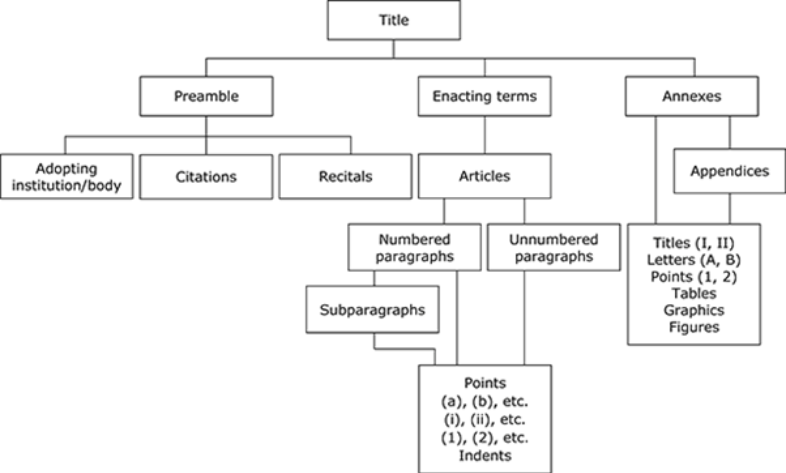
\includegraphics[width=\linewidth]{Images/EU_doc_struct.png}
  \caption{Structure of an act \cite{eu_style_guide_2023}}
  \label{fig:euDocStruct}
\end{figure}

\section{Related work}

The following subsections approach \ac{AI} in the context of this work. It is important to note that this work builds on builds on the value created by a previous dissertation, ``Conceptual Modelling of Legal Compliance Requirements - The cases of eIDAS2 and NIS2''. This provided a methodical and structured approach, composed of four main steps: The creation of an Excel Traceability Matrix as an external legal reference; Developing an ArchiMate Index for internal architectural navigation; Connecting both through a hierarchical numbering system, and Constructing the \ac{AD}s according to the defined architectural principles.

\subsection{\ac{AI} in Regulatory Analysis and Modelling}

Requirements engineering has progressively moved from manual methods towards automated support intended to reduce effort, time, and human error. Early automated approaches focused primarily on requirements analysis, using \ac{NLP} techniques such as part-of-speech tagging and syntax parsing to generate \ac{UML} models and perform consistency checks \cite{Umar2024}. However, such approaches struggled with the ambiguity and contextual complexity of real-world legal documents \cite{Zadenoori2025}.

Generative \ac{LLM}s extend this automation to requirements elicitation, validation, and modelling by synthesising content rather than only detecting or classifying defects \cite{Zadenoori2025}. Their outputs may nevertheless be unreliable when relevant context is unavailable. \ac{RAG} addresses this limitation by retrieving information from enterprise knowledge bases or legal sources to ground model responses \cite{Jeong2023}.

In regulatory \ac{RE}, \ac{MURCIA} uses language models to assist human analysts in identifying and interpreting regulatory changes across textual, semantic, deontic, and pragmatic layers, with an evaluation reporting F1 scores above 90\% for textual and semantic change identification \cite{Abualhaija2024}. Conversational modelling approaches also allow users to describe and iteratively refine model syntax through natural-language interaction \cite{Haerer2023}. Nevertheless, current work remains insufficiently integrated with complex industrial and multi-regulatory workflows, leaving a need for systematic methods that connect regulatory analysis with formal \ac{EA} representations \cite{Zadenoori2025,Elahidoost2024}.

\subsection{Multi-Agent Debate}

\ac{MAD} is a collaborative reasoning approach in which multiple \ac{LLM} agents analyse the same problem, exchange and challenge arguments, and produce a collective conclusion. By making disagreement explicit, it aims to improve accuracy, reduce individual bias, strengthen factual grounding, and provide clearer justification for the final output \cite{oriol2025mad,gomez2026structured}. Its design involves the selection of participants and roles, the interaction mechanism through which agents exchange information, and an agreement mechanism such as voting, scoring, or a judge-based decision \cite{oriol2025mad}.

Independent initial assessments can preserve genuine differences of interpretation before agents are influenced by competing arguments. Later rounds allow agents to rebut, refine, or withdraw their positions; however, additional rounds also increase execution time, token consumption, and cost, often with only marginal gains \cite{oriol2025mad}. Structured approaches organise this process into initialization, argumentation, adjustment, and synthesis, with a moderator controlling turn-taking, preserving debate history, and resolving or recording remaining conflicts \cite{gomez2026structured}.

This work applies \ac{MAD} to regulatory-relevance assessment. Differentiated evaluators analyse legal relevance from literal, systemic, and gap-oriented perspectives, while a moderator records and challenges their reasoning. Explicit consensus is required for inclusion, whereas unresolved cases are preserved for human review, supporting conservative and traceable relevance decisions.

\section{Problem Analysis}

A normative act may affect many organisational units, systems, processes, and governance mechanisms, making a regulation-wide architectural representation too broad for an individual stakeholder. Stakeholders therefore require views that foreground the responsibilities and dependencies relevant to their own work, rather than a universal representation containing substantial irrelevant detail \cite{KosenkovEtAl2025,BreauxEtAl2008}. ISO/IEC/IEEE 42010 and ArchiMate address this need through viewpoints and views, which define and present architectural information for specified stakeholders and concerns \cite{ISO42010:2022,opengroup}. The resulting artefacts must consequently be comprehensible to their intended stakeholders (\textbf{R1}).

This requires bridging a legal-to-operational relevance gap. European legislation, including \ac{DORA}, generally assigns duties to regulated entities, management bodies, or other legally defined roles rather than to individual employees \cite{DORA}. Legal requirements must therefore be related to a stakeholder's documented responsibilities, activities, systems, dependencies, and concerns. This is an interpretative \ac{RE} activity because legal and operational sources use different levels of abstraction, terminology, and perspectives \cite{Ghanavati2014}.

\ac{GenAI} can support this work by structuring legal and operational information, identifying candidate relationships, and producing material for review \cite{Abualhaija2024}. It cannot, however, serve as legal, operational, or architectural evidence: hallucinations and non-deterministic outputs may produce unsupported conclusions \cite{NISTGenAI2024}. The methodology therefore requires human approval (\textbf{R2}), stable results (\textbf{R3}), traceability to legal sources (\textbf{R4}), to operational evidence (\textbf{R5}), and prohibits unsupported inference (\textbf{R6}). These requirements provide criteria for examining the method and its outputs, and are summarized in \ref{tab:requirement-assessment-criteria}. The demonstrations provide preliminary evidence against these criteria. 
Human reviewers inspect, reject, and approve material conclusions, preserving accountability while using \ac{GenAI} as a controlled analytical aid rather than an autonomous compliance assessor.

\begin{table*}[!t]
  \caption{Assessment Criteria for the Methodology Requirements}
  \label{tab:requirement-assessment-criteria}
  \centering
  \small
  \begin{tabularx}{\textwidth}{@{}p{3.5cm}X@{}}
    \toprule
    \textbf{Requirement} & \textbf{Proposed assessment criterion} \\
    \midrule
    R1 --- Comprehensibility &
    Stakeholders can explain represented responsibilities and dependencies and identify omissions or inaccuracies. \\
    R2 --- Human approval &
    Consequential inclusion and modelling decisions have recorded human approval. \\
    R3 --- Stability &
    Repeated executions with unchanged inputs produce materially consistent relevance, ownership, and relationship decisions. \\
    R4 --- Legal traceability &
    Each represented legal duty resolves to an identifiable provision in the selected legal source. \\
    R5 --- Operational traceability &
    Each represented operational claim or relationship is supported by documented stakeholder evidence. \\
    R6 --- Evidence discipline &
    Unsupported claims remain excluded or explicitly unresolved instead of being incorporated as established facts. \\
    \bottomrule
  \end{tabularx}
\end{table*}
\

\section{Methodology}

The methodology goes through 12 stages, ranging from the initial prompt optimization to the delivery of a fully informative model. These are identified as the corresponding number in the following subsections. Multiple agents work throughout every step, making use of a plethora of skills that provide the necessary knowledge basis and restrict \ac{LLM} behaviour. Throughout all the stages, the \ac{LLM} questions the user when it feels it does not have all the necessary information (to prevent hallucination, bolstering \textbf{R6}), and before any decision is locked in, ensuring human approval through-out the process (\textbf{R2}).

To understand the human interactions with the methodology, it is crucial to understand the roles that interact with it. The user is the person who runs the methodology and approves progression between stages while the stakeholder supplies operational knowledge and comments on whether the resulting representations reflect their work.

\subsection{Traceability Matrix Evolution}

The Excel Traceability Matrix evolved from a manual process to a fully automated one. A program was created to analyse the \ac{HTML} from the target legislation, and output the Traceability Matrix without any human input.

Besides automation for the sake of efficiency, the traceability matrix also suffered a complete redesign to improve readability (\textbf{R1}). The baseline Traceability Matrix used an \ac{ID} system that was not intuitive. This is because the different \ac{ID}s can refer to any of the sub-article levels, which are not explained anywhere in the matrix. Additionally, of all the groupings referred in section \ref{sec:legisStruc}, only Chapters are mentioned. To address this, every possible grouping that a a legislative text may have exists as an \ac{ID} column (\textbf{R4}). An excerpt of the new traceability matrix can be observed in table \ref{tab:newTraceMatrix}.

\begin{table*}
    \caption{Sample from the traceability matrix of \ac{DORA} generated by the traceability matrix creator program}
    \centering
    % Use \includegraphics to load the screenshot of your table
    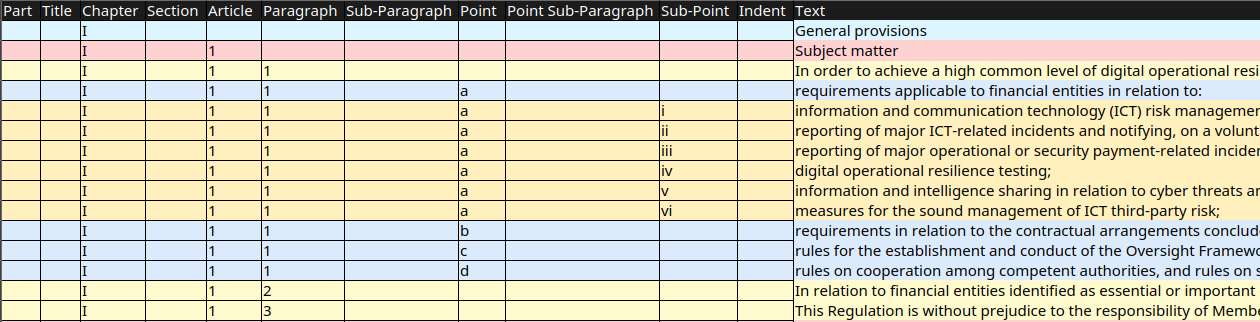
\includegraphics[width=1\linewidth]{Images/DoraTraceMatrixExcerpt.png} 
    \label{tab:newTraceMatrix}
\end{table*}

\subsection{Context Discovery}

The twelve phases of the methodology are organised into three groups. The first, Context Discovery, comprises stages one to five and establishes the evidence base required for later viewpoint scoping and materialisation.

\textbf{1 - }The first stage, Prompt Optimization, converts the initial user request into a bounded and unambiguous pipeline input. It preserves the intended objective, introduces explicit constraints, and records missing information as placeholders rather than supplying assumptions. The approved prompt is retained as an artefact, ensuring that the initial scope and subsequent decisions remain visible throughout the methodology (\textbf{R6}).

\textbf{2 - }Interview Design then produces a jargon-free and regulation-blind interview guide for eliciting the stakeholder's operational footprint (\textbf{R1}). Questions address the stakeholder's mission, workflows, assets, dependencies, resilience practices, and governance context, supported by alternative angles and fallbacks. The user conducts the interview and records the responses, producing the documented operational evidence required by the following stages (\textbf{R5}).

\textbf{3 - }The third stage, Operational-Footprint Extraction, analyses the interview responses and records distinct operational facts using \texttt{OP-*} identifiers. Explicit relationships are separately captured as \texttt{REL-OP-*} records, including their endpoints, direction, and supporting interview evidence (\textbf{R5 and R6}). Tasks, assets, dependencies, approvals, incident interfaces, and friction points are reviewed and approved separately.(\textbf{R2})

\textbf{4 - }Stakeholder and Concern Identification uses the approved operational footprint to determine the stakeholder's organisational position and identify every documented concern, bottleneck, friction point, or operational gap. Each concern receives a \texttt{CON-*} identifier and, where available, retains its originating \texttt{OP-*} evidence (\textbf{R5}).

\textbf{5 - }Regulatory Relevance Analysis is the fifth stage and evaluates the approved operational footprint, stakeholder classification, and concerns against the selected \ac{EU} legislation. Three evaluators independently assess the legal text from literal, systemic, and gap-oriented perspectives, retrieving and analysing the regulation article by article. Each candidate article must be justified through an operational anchor, a legal bridge, and an ownership assessment (\textbf{R5 and R6}). A moderated debate then takes place to attempt to resolve disagreements. Only unanimously accepted articles proceed as relevant, while unresolved cases remain visible for user review, supporting stable relevance decisions (\textbf{R3}).

For each approved article, the process records atomic legal duties as \texttt{REQ-*} requirements and resolves them against verified canonical legal-text identifiers in the generated traceability matrix (\textbf{R4}). A Coverage Ledger then connects requirements to documented \texttt{OP-*} or \texttt{CON-*} records through \texttt{COV-*} entries. The resulting \texttt{REL-COV-*} relationships record the operational and legal endpoints, supporting evidence, effect, and ownership state, thus preserving traceability to operational evidence and preventing unsupported relationships (\textbf{R5}, \textbf{R6}).

Finally, the process maps the stakeholder through the employing organisation to the applicable law-defined entity or role group through evidence-backed \texttt{REL-ROLE-*} relationships (\textbf{R5}). This distinction prevents an individual employee from being incorrectly represented as the regulated entity. The resulting report is approved through gates covering article selection, omitted candidates, legal anchors, coverage relationships, and legal-role placement, becoming the approved evidence base for the next methodological group (\textbf{R2}).

\subsection{Viewpoint Definition}

The second group of the methodology comprises stages six to eight and converts the approved evidence base into a formal stakeholder viewpoint. It begins with a technology-selection gate, in which the user selects the technology used to materialise the immutable regulation overview baseline (\textbf{R2}).

The regulation overview and the stakeholder-specific views have different scopes. The overview is derived from the complete binding text within the selected legal corpus and preserves the regulation-wide legal context. Stakeholder-specific views are subsequently derived from the narrower set of duties and operational relationships justified by the relevance and coverage analysis (\textbf{R5 and R6}). 

\textbf{6 - }Three technology choices are available. Direct ArchiMate \ac{XML} generation produces a native \texttt{.archimate} model that can be opened in Archi; LikeC4 provides an experimental architecture-as-code alternative based on a concise \ac{DSL}, although its primary scope is software rather than enterprise architecture; pyArchimate generates an ArchiMate model through a Python script. Regardless of the technology selected, the overview retains the same legal core (\textbf{R3}): Binding duties are organised into requirement families, anchored to verified legal text  (\textbf{R4}), connected to the \texttt{'stakeholder'-'organisation'- 'legal-role'} chain, validated for connectivity, and approved before later stages may use it.

\textbf{7 - }Viewpoint Scope determines which approved legal and operational material should be represented for a stakeholder, and why. Ownership remains explicit, distinguishing work directly performed by the stakeholder from externally owned, constrained, or unclear controls (\textbf{R6}). The user approves the boundary, included requirements, streams, and connectivity of the proposed views (\textbf{R2}).

\textbf{8 - }Viewpoint Generation converts the approved scope into a formal ArchiMate viewpoint specification. For each proposed view, it defines its purpose, stakeholder perspective, concerns, operational streams, permitted ArchiMate concepts and relationships, requirement-family structure, and visual rules (\textbf{R1}). The regulation overview remains unchanged as the regulation-wide legal baseline (\textbf{R3}), while the additional views represent the narrower stakeholder-specific scope.

This stage also produces \texttt{7\_view\_graph.json}, an authoritative machine-readable contract for later narrative, slide, and model generation. It records every permitted node, approved \texttt{REL-*} relationship, evidence reference, ownership safeguard, requirement-family nesting rule, and stakeholder anchor for each view (\textbf{R5}). The user validates both the ArchiMate metamodel rules derived from the approved scope and the complete view graph before the viewpoint specification and graph are persisted, supporting stable and evidence-traceable later artefacts (\textbf{R3, R4 and R5}).

\subsection{View Generation}

The final methodological group comprises stages nine to twelve and materialises artefacts that communicate how the selected legislative act affects the operational footprint of the stakeholder. The produced artifacts are a textual explanation (phase 9), markdown diagrams (phase 10), and ArchiMate views (phase 11).

The approved view graph is the reference against which generated artefacts are checked. It records the permitted elements, relationships, ownership states, and evidence references. Conformance to this graph establishes consistency with the approved specification (\textbf{R3}).

\textbf{9 - }Textual View Explanation produces a per-view narrative from the approved viewpoint and view graph. It explains the regulatory and operational context of each view and how its elements and relationships should be interpreted (\textbf{R1}). The resulting explanation also includes a traceability table connecting coverage entries to their operational evidence, legal requirements, ownership states, and representing elements (\textbf{R4 and R5}). The user approves each view name and description (\textbf{R2}).

\textbf{10 - }Markdown Slide Diagrams provide a condensed, presentation-oriented representation of the overview and each stakeholder-specific view. Each slide contains an \texttt{ASCII} sketch of the principal operational path, dependencies, and requirement families, supported by tables listing granular requirements and approved relationships. The slide is therefore meant to be an accessible summary rather than a complete graphical projection of the underlying view graph, and is accompanied by a plain-language operational takeaway (\textbf{R1}). Each slide and its supporting information require user approval before persistence (\textbf{R2}).

\textbf{11 - }View Generation then materialises the approved viewpoint as a native architecture model that can be opened, inspected, reused, and refined. The selected technology (direct ArchiMate \ac{XML}, LikeC4, or pyArchimate) receives the regulation overview, viewpoint specification, authoritative view graph, explanation, and slides. The view graph remains the source of truth (\textbf{R3}), while the narrative and slides support the organisation and presentation of the native model.

The generator creates all approved model elements and relationships while preserving requirement-family containment, stakeholder anchors, ownership safeguards, and legal documentation (\textbf{R4}). A stakeholder is represented as realising a requirement only when the relevant work is directly performed. Otherwise, dependencies, constraints, approvals, or external roles are represented instead. The output is validated against the selected technology and reconciled with the view graph: missing or additional elements, altered relationships, broken containment, disconnected views, or changes to the overview cause rejection (\textbf{R3 and R6}). Proposed layouts are presented to the user for approval before the model is saved (\textbf{R2}).

\textbf{12 - }Lastly, Cross-Artifact Reconciliation verifies that the overview, viewpoint and graph, textual explanation, slides, native model, and legal traceability matrix communicate the same approved information (\textbf{R3}). Using the graph as the ground truth, it checks legal anchors, operational chains, view membership, relationships, ownership semantics, containment, and technology-specific model validity (\textbf{R4, R5 and R6}). Any discrepancy is documented in an audit report and corrected only after user approval, after which the audit is repeated (\textbf{R3}). This ensures that the different artefacts can support different readers without silently communicating incompatible regulatory or operational claims.

\section{Results and Demonstration}

The method was demonstrated with two banking stakeholders: a back-end developer and an infrastructure and cloud engineer with database-administration responsibilities. These cases illustrate different operational contexts within the same regulatory domain, covering software delivery and technical platform administration. Feedback was collected during presentations of the generated views and explanatory artefacts to the stakeholders. The observations provide qualitative evidence of usefulness and limitations within these cases.

\subsection{Operational Context}

Both cases began with an optimised prompt and a stakeholder interview used to establish the operational footprint and analysis boundary. In the back-end developer case, the prompt retained placeholders to delimit the available context and objectives, whereas the Infrastructure and Cloud Engineer prompt was considered sufficiently complete without them. Both were used to produce an interview to be conducted with the designated stakeholder by the user. The infrastructure interview was sent to the stakeholder instead of being conducted, resulting in the feedback that some questions were vague. Nevertheless, the responses provided sufficiently detailed information.

For the back-end developer, the analysis boundary concerns work on an internal Data Platform. The stakeholder develops varied services as well as framework changes, code tests, creates pull requests, coordinates releases and monitors production deployments. Their work depends on functional specifications, permissions, management and solution-architecture decisions, infrastructure deployment support, cloud-native infrastructure and core platform services. The resulting footprint contains 89 approved, interview-grounded records. The stakeholder accepted the extracted footprint, classification, and concerns without amendment.

For the Infrastructure and Cloud Database Administrator, the boundary concerns the administration of distributed query engines, metadata management, and high-performance databases within the bank's internal data-technology layer. The stakeholder provisions access, maintains technologies through updates and configuration changes, validates deployments, investigates connection and usage problems, and supports incident response. Their work depends on infrastructure, networking, technology-support, security, and authorisation teams, as well as enterprise platforms for access governance, release automation, security management, observability, and \ac{IT} service operations. This case produced 58 approved operational records, whose footprint and concerns the stakeholder considered accurate.

Both boundaries distinguish technical work directly performed by the stakeholder from decisions and controls owned elsewhere. The developer implements and tests changes but lacks final authority for architecture, functional requirements, and production approval. The infrastructure stakeholder remains constrained by DevOps-change, access, and production-authorisation processes. Both participate in incident handling within defined escalation paths, although the infrastructure stakeholder also restarts, investigates, and mitigates database outages before producing a post-incident report. These distinctions provide the evidence base for subsequently determining which regulatory effects can be attributed to the stakeholder, represented as external constraints, or excluded from the viewpoint.

\subsection{\ac{DORA} Relevance and Ownership}

In both cases, regulatory relevance analysis compared the approved operational footprint with \ac{DORA} through the multi-agent debate panel. Rather than treating every entity-level duty as a personal stakeholder responsibility, the analysis retained only requirements supported by an operational chain and recorded their legal anchors and ownership states. This enables the resulting views to distinguish controls directly performed by the stakeholder from constraints, external dependencies, and responsibilities for which the available evidence does not establish an owner.

In the back-end developer case, the selected \ac{DORA} scope concentrated on duties affecting platform development, controlled change, testing, monitoring, continuity, and incident-related work. Duties concerning the wider \ac{ICT} risk-management framework, crisis communication, incident classification, and reporting to competent authorities were excluded because the interview did not evidence developer participation. A deliberate manual addition of Article~28 was used to test intervention in the relevance process. The resulting cloud-risk material remained weak because the evidence did not establish a direct effect on the developer's work, demonstrating that the method retains the distinction between legal applicability to the bank and relevance to an individual stakeholder.

For the Infrastructure and Cloud Engineer case, the panel selected a broader set of requirements spanning the \ac{ICT} risk-management lifecycle, including platform administration, access and security, controlled change, monitoring, recovery, incident handling, and resilience testing. This wider scope reflected the stakeholder's documented responsibility for configuring and maintaining core data query, governance, and storage platforms, as well as supporting access management, testing, incident response, and service recovery. In contrast, management-body governance, authority reporting, and entity-level third-party-risk management remained outside the stakeholder boundary because they were not evidenced as part of the role.

The two cases therefore produced different relevance boundaries while applying the same evidence and ownership rules. The developer viewpoint emphasised the delivery lifecycle and its dependencies on decisions and controls owned by other teams, whereas the Infrastructure and Cloud Engineer viewpoint covered a broader technical-administration and resilience context. In both cases, pyArchimate was selected to produce the overview model, but the distinct operational evidence resulted in different requirement-family structures. The resulting views preserve the wider \ac{DORA} legal context while limiting direct stakeholder responsibility to what the operational evidence supports.

\subsection{Resulting Architecture Description}

Both stakeholder cases produced pyArchimate \acp{AD} from approved viewpoints, preserving the regulation overview, legal requirements, operational evidence, ownership states, and ArchiMate relationships. In each case, the architecture description separates work directly performed by the stakeholder from external organisational controls, dependencies, and areas where ownership could not be established. The resulting models are therefore intended as traceable communication and refinement artefacts rather than as assessments of organisational compliance.

For the back-end developer, the resulting \ac{AD} contains the regulation overview and six stakeholder-specific thematic views: \ac{ICT} Asset Governance, Protection and Change, Detection and Continuity, Incident Learning, Resilience Testing, and Microsoft Cloud Risk. This structure reflects the developer's delivery-oriented operational boundary, connecting development, testing, release, monitoring, and incident work to the relevant \ac{DORA} constraints.

The Resilience Testing view in Figure~\ref{fig:dora-resilience-testing} illustrates a positive outcome of the developer case. It represents developer testing and readiness activities, pull-request creation, and the separate Technical Reviewer role. Requirements directly supported by the developer's work are distinguished from review responsibilities for which the interview did not establish ownership, making visible both direct contribution and external constraint.

\begin{figure}[H]
  \centering
  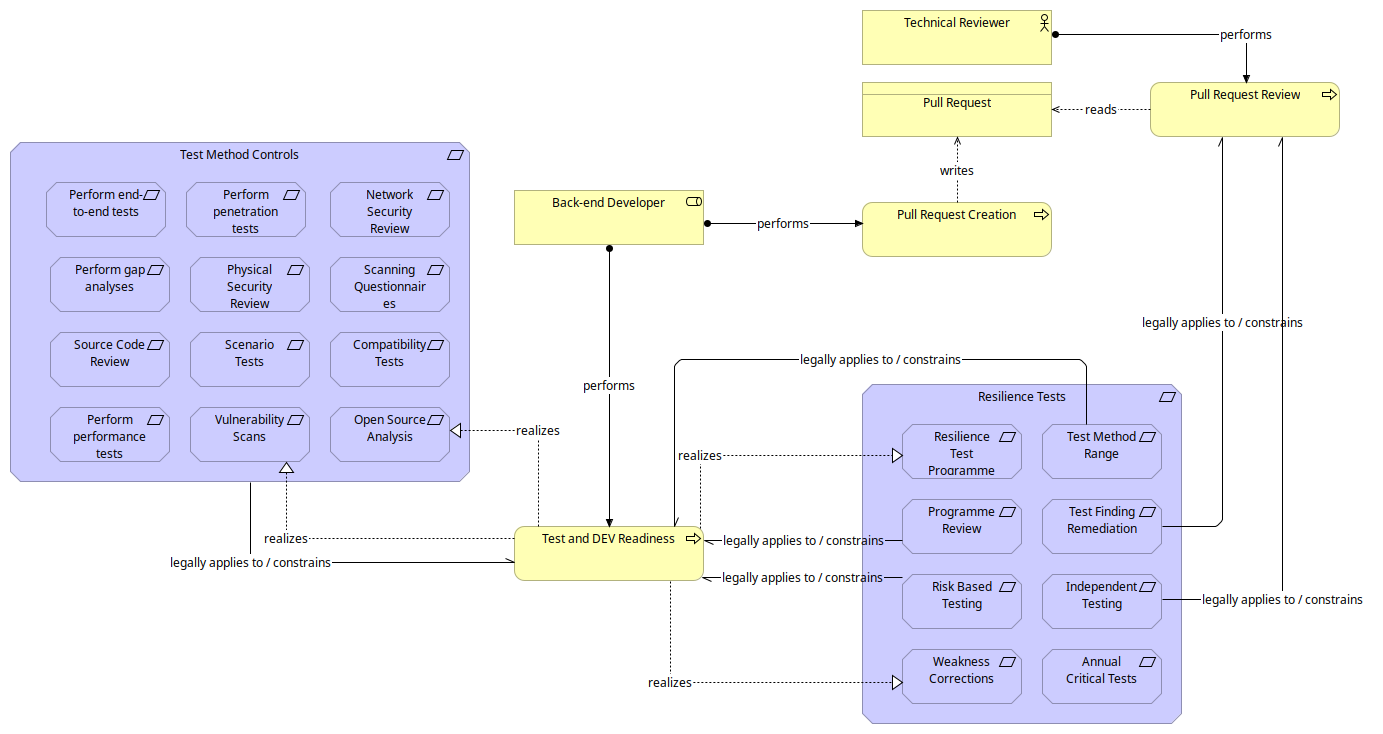
\includegraphics[width=\linewidth]{Images/dora-resilience-testing.png}
  \caption{\ac{DORA} Bank Developer Resilience Testing View}
  \label{fig:dora-resilience-testing}
\end{figure}

The Microsoft Cloud Risk view in Figure~\ref{fig:dev-microsoft-cloud-risk} provides an important result. It was generated after Article~28 was manually included in the relevance analysis, despite the absence of evidence that the developer's work was affected by a Microsoft contract or related third-party-risk duties. The resulting weak view demonstrates that the method did not invent a stakeholder responsibility merely to make the view appear complete: the relevant responsibility belongs to the employing entity rather than to the developer.

\begin{figure}[H]
  \centering
  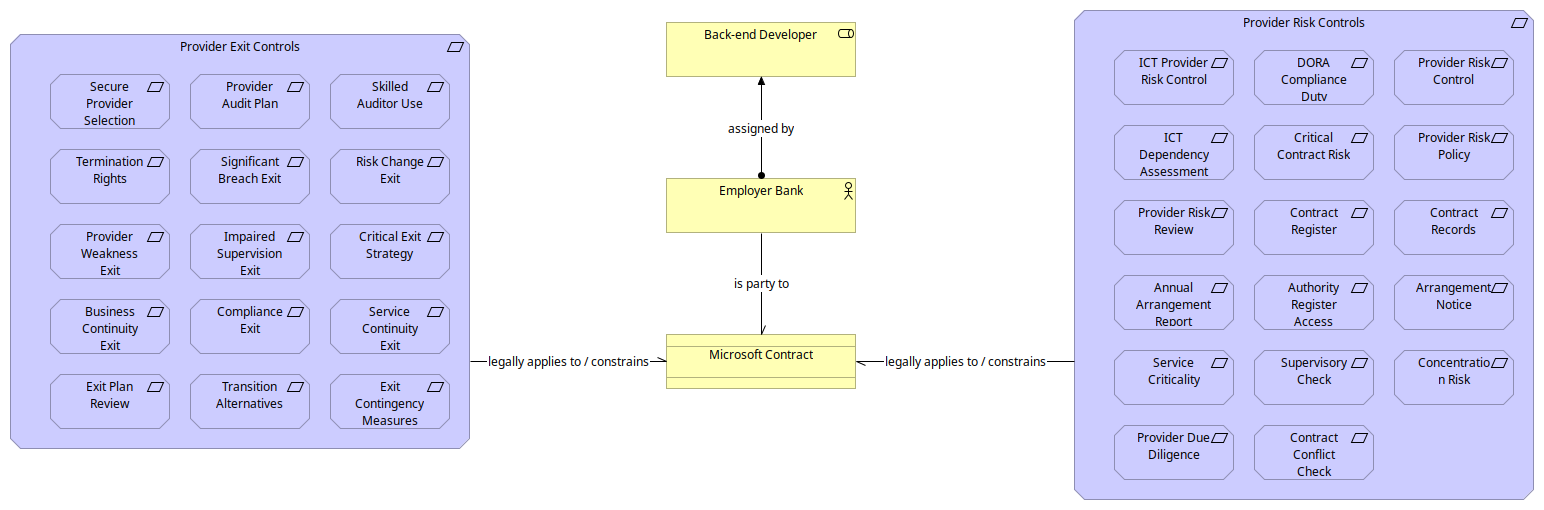
\includegraphics[width=\linewidth]{Images/Dev_Microsoft_Cloud_Risk.png}
  \caption{\ac{DORA} Bank Developer Microsoft Cloud Risk View}
  \label{fig:dev-microsoft-cloud-risk}
\end{figure}

The Infrastructure and Cloud Engineer case produced a broader \ac{AD} comprising seventeen connected views: the immutable \ac{DORA} overview, thirteen legal thematic views, and three operational-context views. The legal views address topics such as platform and asset management, access and security, controlled change, monitoring, recovery, incident management, and resilience testing. The three operational context views preserve relevant colleague support, investigation tooling, and emergency change evidence that could not defensibly be connected to a specific \ac{DORA} requirement.

Figure~\ref{fig:controlled-change-view} presents the Infrastructure and Cloud Engineer's Controlled Change view. It represents the approval path for a production change and the dependencies that constrain the stakeholder's ability to alter technologies in production. The stakeholder considered this view accurate while identifying possible improvements, providing preliminary evidence that the architecture description was sufficiently understandable to support stakeholder feedback and later refinement.

\begin{figure}[H]
  \centering
  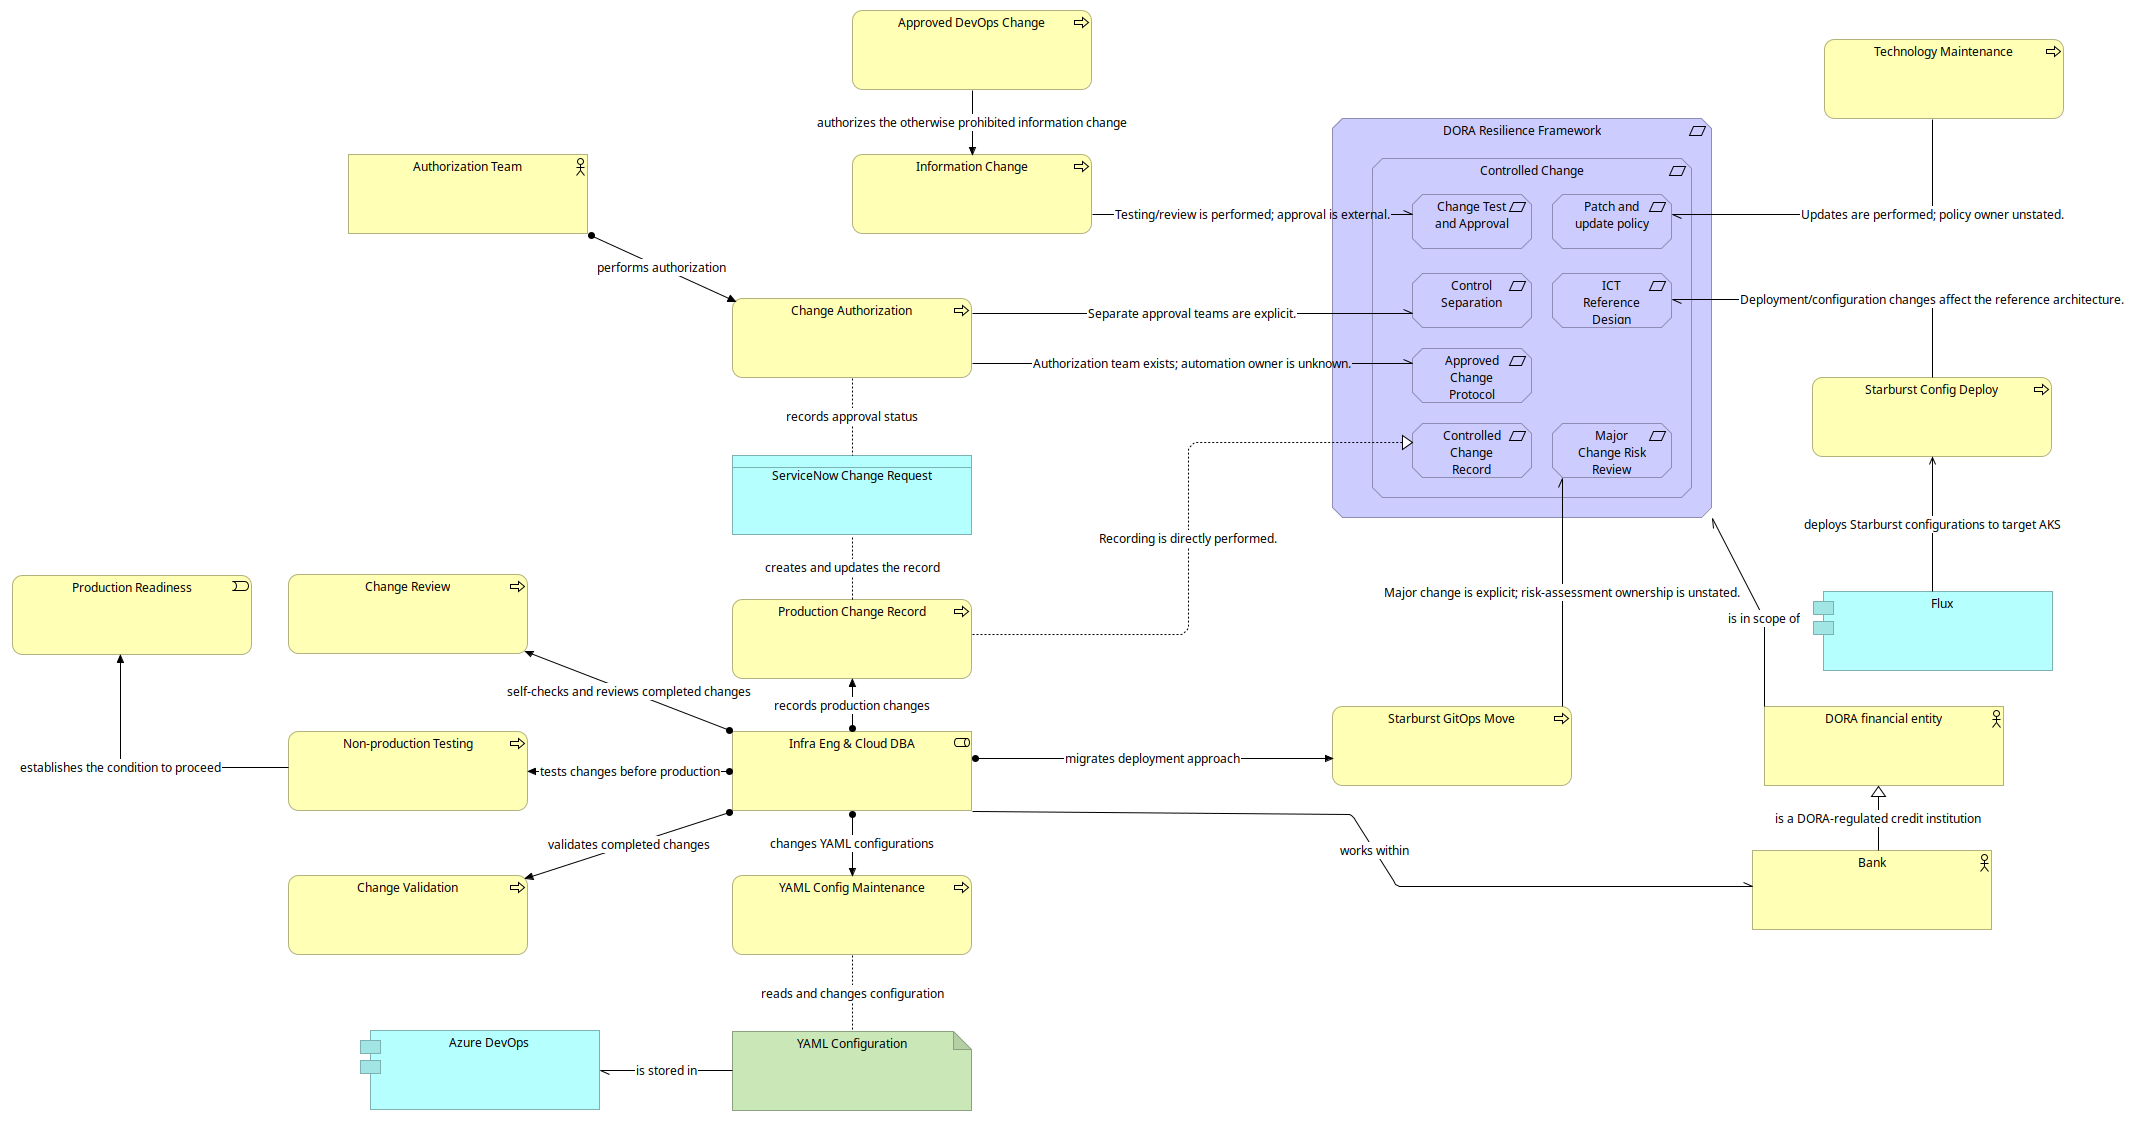
\includegraphics[width=\linewidth]{Images/Controlled Change.png}
  \caption{\ac{DORA} Infrastructure and Cloud Engineer Controlled Change View}
  \label{fig:controlled-change-view}
\end{figure}

The contrast between the cases reflects their different operational roles. The developer description is narrower and centred on the software-delivery lifecycle, whereas the Infrastructure and Cloud Engineer description spans a broader set of technical, administration and resilience responsibilities. Correspondingly, the developer viewpoint contains six thematic views and exposes substantial dependencies on externally owned controls, while the infrastructure viewpoint contains thirteen legal views and separate operational-context views for activities without a defensible direct legal effect.

Both cases were complemented by textual explanations and condensed Markdown slide diagrams. The textual explanations provide a per-view walkthrough of elements and relationships, while the slides offer simplified visual summaries. However, the developer case showed that these supplementary artefacts did not yet consistently achieve their intended accessibility objectives, and the simplified slides risked omitting context needed to convey the full regulatory and operational meaning. The formal ArchiMate views therefore remain the principal artefacts, with explanatory material requiring further refinement to provide stronger stakeholder-oriented support.

\section{Conclusion}

The \ac{DORA} demonstrations support the feasibility of deriving stakeholder-specific viewpoints and ArchiMate views from documented operational evidence and binding legal requirements. The extracted footprints and concerns reflected stakeholder accounts, while relevance analysis identified applicable articles, decomposed their requirements, and preserved legal and operational traceability. Preliminary feedback indicated that the formal views supported regulatory understanding and identification of omissions. However, the secondary objective was only partially achieved, as narratives and simplified diagrams provided inconsistent explanatory support.

These outcomes should be interpreted within the scope of the demonstrations. \ac{GenAI} supported the extraction, organisation, and representation of information, but human review, approval gates, traceability, and cross-artifact reconciliation remained necessary to constrain its use. Moreover, the completeness of a viewpoint depends on the information made explicit during elicitation: omitted activities or controls may remain unrepresented or have unclear ownership. The generated views can therefore serve not only as communication artefacts, but also as feedback mechanisms through which stakeholders identify omissions and enrich subsequent iterations. Broader assessment with additional stakeholders and independent reviewers remains necessary.

Future work should improve the presentation and explanation of generated views. Although the current models are structurally valid, their layout still requires manual refinement to improve readability, reduce relationship crossings, and better reflect stakeholder reading paths. Automated layout and connector-routing strategies could reduce this effort. Textual explanations should also move beyond describing the methodology itself and instead explain the regulatory and operational significance of the view from the perspective of the stakeholder.

The methodology could also be extended in its legal and technical foundations. Incorporating \ac{RTS} and \ac{ITS} would enable the method to represent more detailed obligations concerning areas such as \ac{ICT} change management, testing, source-code testing, and logging. Further work is also needed to improve traceability-matrix parsing and identifier schemes for amendment-heavy legislation, as well as to update the pipeline for ArchiMate~4.

Beyond stakeholder communication, the methodology could support enterprise gap detection and version-aware regulatory analysis. Comparing viewpoints obtained from multiple employees, particularly across equivalent roles, could reveal recurring indications of organisational gaps that warrant review, although a single interview cannot establish non-compliance. Recording regulatory versions and effective dates could additionally enable the method to identify which requirements, viewpoints, and models are affected by later legal amendments, allowing targeted maintenance rather than repetition of the complete pipeline.

%%
%% The next two lines define the bibliography style to be used, and
%% the bibliography file.
\bibliographystyle{ACM-Reference-Format}
\bibliography{bibliography}

\end{document}
\endinput
%%
%% End of file `acmtog.tex'.
